\documentclass[conference]{IEEEtran}

\usepackage[fleqn]{amsmath}
\usepackage{algpseudocode}
\usepackage{graphicx}
\graphicspath{ {images/} }
\interdisplaylinepenalty=2500
\hyphenation{op-tical net-works semi-conduc-tor}

\begin{document}
\title{Parallel Bat Optimization on GPU using CUDA}

\author{\IEEEauthorblockN{Jean Carlo Machado}
\IEEEauthorblockA{Univerisdade do Estado de Santa Catarina\\Mestrado de Computação Aplicada\\
UDESC\\
Santa Catarina, Joinville,\\
Email: contato@jeancarlomachado.com.br}
\and
\IEEEauthorblockN{Rafael Stubs Parpinelli}
\IEEEauthorblockA{Univerisdade do Estado de Santa Catarina\\ UDESC\\
Santa Catarina, Joinville
}}

\maketitle

\begin{abstract}
The ever increasing parallel processing power of GPU's is an compelling
motive to implement performance demanding algorithms, like optimization
techniques, using this technology. This work aimed to develop a GPU
version of the bat metaheuristic, a CPU version were developed as well,
as a way of comparison. A set of experiments where conducted in order
to measure the speedup difference. The results suggests that the GPU
version is able to achieve relevant speedups in highly populational
problems but for simpler cases the CPU version might outperform GPU.
\end{abstract}

\IEEEpeerreviewmaketitle

\section{Introduction}%{{{

With the aid of parallel computing, specially GPU computing, it's
possible to tackle ever increasing computational problems in decreasing amounts of time.
A good way of solving complex problems, like NP one's is through the use
of optimizaton algorithms, specially meta-heuristics. In the group of
meta-heuristics a promising field for parallel computings is the swarm
intelligence group. Which encompases many bio-inspiratons liks PSO, ACO,
BAT, etc.

Parpinelli \cite{newInspirations}, when reffering to swarm
intelligence algorithms, define that they are: \begin{quote} compounded by a distributed
society/population of individuals where the control is also
distributed among the individuals (there is no centralized control);
and the individuals decision-making is stochastic and based only on
local information .\end{quote}

The fact that swarm intelligence algorithms have composable that run
conceptually independent from one another makes them ideal for parallel
enviroments.

This work attempts to investigate the applicability of a relatively new
and promising swarm algorithm: the BAT algorithm in the GPU using CUDA.
Previously some demonstrations of the bat algorithm parallelized on CPU
were presented in \cite{paralellCPUFirst} and \cite{paralellCPU}. A
novel publication about the use of the bat optimization can be found on
\cite{firstBatGPU}.

However no case was used til this moment to the applicability of the bat on gpu when comparing standard benchmark functions.

The rest of the paper is organized as following: section \ref{cuda}
gives a overview of cuda and its components. Section \ref{bat}
studies the bat meta-heuristic, it's design and details. Section
\ref{experiments} details the experiments performed. Section
\ref{results} analyses the results and concludes.

%}}}

\section{Cuda} \label{cuda}%{{{

Compute Unified Device Architecture (CUDA) is a general purpose
parallel computing programming model for parallel computations \cite{cudaDefinition}. CUDA
uses a SIMD \textit{single data multiple execution} approach \cite{cuda_optimizations}, where the
concurrent code executes the same instruction but with divergent data.

%%how cuda is organized?

The basic element of work in a cuda device is a thread. That is aggrouped and 
runs in parallel with 32 other threads called the warp.
Wraps are grouped in blocks.


\begin{figure}
    \begin{center}
    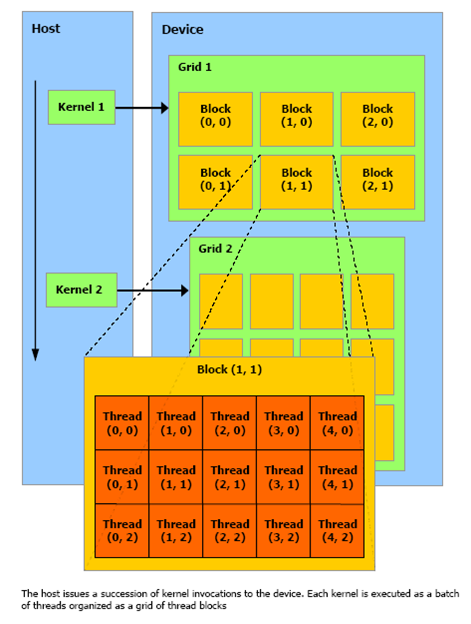
\includegraphics[width=200px,height=200px]{cudaModel}
    \end{center}
    \caption{The cuda structural organization}
\end{figure}

%%how is cuda execution model

A cuda program starts by allocating resources on the GPU and
dispatching work to de done on the GPU.

Once the GPU finishes it's work the GPU they are moved back from GPU
memory to the CPU one. And the results can be returned.

For the developer, the basic element of concern is the kernel, which is the function
executed on the GPU. A kernel function defines the code to be executed by each of the massive
numbers of threads to be invoked \cite{gpuOptimization}.

%% some concerns of optimizing applications in cuda
\subsection{Performance concerns in CUDA}
Since the cuda model is complex, it's not trivial to setup an ideal configuration 
of a problem in the GPU. However many good practises exists and great speedup is already 
reported.  Previous researches suggests that highly parallel
applications may speedup up to 450 times \cite{gpuOptimization}.

Below are described some of the major concern while developing parallel algorithms  in CUDA.

\begin{itemize}
    \item When attempting to achieve an application's maximum performance, the primary concern often is managing global memory latency \cite{cuda_optimizations}. It's preferable to use local memory and shared memory instead of global since they are much faster.
    \item In an ideal enviroment when the GPU starts
        working the less the messaging passing between the GPU and the CPU, the better.
    \item Decrease data interchange between the host and the GPU to the mininum.
    \item Prefer floats to doubles when possible. The older versions of
    CUDA GPU's had serious bottlenets using large variables type, but
    this is a issues disappearing
\end{itemize}

%}}}

\section{Bat algorithm} \label{bat} %{{{

The bat algorithm is a populational meta-heuristic introduced by Yang in
2010. It uses the inspiration of micro-bats which uses a type of sonar,
called echolocation, to detect prey, avoid obstacles, and locate their
roosting crevices in the dark \cite{original}.

The bat algorithm has two paramters: the pulse rate and the loudness.
As time goes by the pulse-rate tends to increase and the loudness to
decrease. The inspiration comes from the behaviour of bats that uses
pulse rate as a slow and loud while in search for a pray and quick
and low pitches when in perseguition of one. In the bat algorithm the
loudness is used as a way of accepting bad results (diversification) and
pulse rate as a way of selecting local search (exploitation).

\subsection{Bat Design on CPU}

The bat original paper don't clarify all the implementation details
working of the algoritm.

In this work the bath algorithm used was the one proposed by
\cite{comparisonBatParpinelli}, since it represents a concrete demonstration of how
the bat metaheuristic might work.

Some distinctions of the original paper are worth noticing

\begin{itemize}
    \item The selection of new results on the original paper tends to be more greedy (line 14) [improve the descritpion of the other paper].
    \item On this paper the or operator were used but in the original one an And were proposed.
    \item The or operator tends to explore the search space better (more diversity).
    \item There's a distortion on a single dimension of the search space in
order to increase the diversity factor.
\end{itemize}

The CPU version developed was single threaded. The random algorithm used
was the xorshift algorithm.

\begin{figure}
\begin{algorithmic}[1]
\State $Parameters:\ n,\alpha,\ \lambda$
\State $initialize\ bats$
\State $evaluate\ fitness$
\State $selects\ best\ \vec{x}_*$
\While {$stop\ criteria\ false$}
    \For{$each\ bat$}
        \State $f_i=f_{min} + (f_{max} - f_{min})\beta, \in \beta [0,1]$
        \State $\vec{v}_i^{t+1} = \vec{v}_i^{t} + (\vec{x}_i^{t} + \vec{x}_*^{t})f_i$
        \State $\vec{x}_{temp} = \vec{x}_i^{t} + \vec{v}_i^{t+1}$
        \If {$rand < r_i, rand \in [0,1] $}
            \State $\vec{x}_{temp} = \vec{x}_* + \epsilon A_m, \epsilon \in [-1, 1]$
        \EndIf

        \State $single\ dimension\ perturbation\ in\ x_{temp}$
        \If {$a < A_i^t\ \textbf{or}\ f(\vec{x}_{temp}) \leq f(\vec{x}_i), a \in [0,1] $}
            \State $\vec{x}_i^t = \vec{x}_{temp}$
            \State $r_i = exp(\lambda * i)$
            \State $A_i =  A_{0} * \alpha^i$
        \EndIf
    \EndFor
    \State $selects\ best\ \vec{x}_*$
\EndWhile
\end{algorithmic}
\caption{Pseudo-code CPU}\label{cpu-pseudo}
\end{figure}

\subsection{Bat Design on GPU}

\begin{figure}
    \begin{center}
    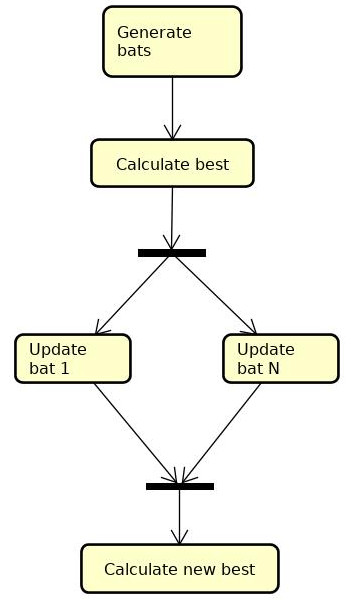
\includegraphics[width=150px,height=200px]{activity}
    \end{center}
    \caption{GPU process flow}
\end{figure}


A conveninet approach to model the swarm in the GPU is to use each
thread as an individual. \cite{pso-gpu} used a similar method for a
GPU implementation for the PSO algorithm, and he says \begin{quote}
Each element of the particle is treated individually in the thread,
allowing efficient data parallelism whitout risk of starvation or race
conditions.\end{quote}

In the bat algorithm synchronization must occur on the selection of the
best individual of the iteration. The best individual is kept in the
threaded memory of the GPU which has a limit of 16KB, probably not feasible for
more complex problems.

The initial random number generator used on the GPU was the MTGP32.
However later was discovered it's not recommended to use more than 256
threads per block with it \cite{curandIssue}. So we moved the algorithms
to the cuda default XORWOR.

\begin{figure}
\begin{algorithmic}[1]
\State $Parameters:\ n,\alpha,\ \lambda$
\State $initialize\ bats\ asynchronously$
\State $evaluate\ fitness$
\State $synchronize\ threads$
\State $selects\ best\ \vec{x}_*$
\While {$stop\ criteria\ false$}
    \For{$each\ thread$}

        \State $f_i=f_{min} + (f_{max} - f_{min})\beta, \in \beta [0,1]$
        \State $\vec{v}_i^{t+1} = \vec{v}_i^{t} + (\vec{x}_i^{t} + \vec{x}_*^{t})f_i$
        \State $\vec{x}_{temp} = \vec{x}_i^{t} + \vec{v}_i^{t+1}$
        \If {$rand < r_i, rand \in [0,1] $}
            \State $\vec{x}_{temp} = \vec{x}_* + \epsilon A_m, \epsilon \in [-1, 1]$
        \EndIf

        \State $single\ dimension\ perturbation\ in\ x_{temp}$
        \If {$a < A_i^t\ \textbf{or}\ f(\vec{x}_{temp}) \leq f(\vec{x}_i), a \in [0,1] $}
            \State $\vec{x}_i^t = \vec{x}_{temp}$
            \State $r_i = exp(\lambda * i)$
            \State $A_i =  A_{0} * \alpha^i$
        \EndIf
    \EndFor
    \State $synchronize\ threads$
    \State $selects\ best\ \vec{x}_*$
\EndWhile
\end{algorithmic}
\caption{Pseudo-code GPU}\label{gpu-pseudo}
\end{figure}

%}}}

\section{Experiments} \label{experiments}%{{{ 

For testing the performance of the algorithm a set of experiments where
developed using diverse benchmark functions tested against a set of
individuals in a highly dimensional problem.

The benchmark functions used were the following:

\begin{itemize}
    \item Ackley
    \item Griewank
    \item Rastringin
    \item Rosenbrook
\end{itemize}

The experiments were executed on a machine with the following configuration:

\textit{Intel(R) Core(TM) i5-4460  CPU @ 3.20GHz \\ GK208 GeForce GT 720 1024 MB of vram \\ Compute capability 3.5 \\ Kepler GM10x}

Each experiment was executed a total of 20 times with 10 thousand
iterations each and 100 dimensions in each function.

\begin{table}[!htbp]
    \renewcommand{\arraystretch}{1.3}
    \caption{Experiments}
    \label{experiments}
    \centering
    \begin{tabular}{c|c|c|c}
    \hline
        \bf Name & Function &  Dimensions & Agents\\
    \hline
        E1 & Ackley & 100 & 256\\
        E2 & Ackley & 100 & 768\\
        E3 & Griewank & 100 & 256\\
        E4 & Griewank & 100 & 768\\
        E5 & Rastringin & 100 & 256\\
        E6 & Rastringin & 100 & 768\\
        E7 & Rosenbrook & 100 & 256\\
        E8 & Rosenbrook & 100 & 768\\
    \end{tabular}
\end{table}

%}}}

\section{Results} \label{results}%{{{

In this section are described the speedup and convergence results. The
time spent in each execution of the algorithms is described in seconds.

%cpu
%ROSENBROOK & 1000 & 128 & 93.2765 & 0.106094 & 12899091640 & 1.11906e+10


\begin{table}[!t]
    \renewcommand{\arraystretch}{1.3}
    \caption{CPU Results}
    \label{results-cpu}
    \centering
    \begin{tabular}{c|c|c|c}
    \hline
        Time Avg & Time SD & Fit Avg & Fit SD\\
    \hline
        (E1) 49.4428 & 0.0557314 & 4.44089e-16 & 2.05196e-22 \\
        (E2) 161.439 & 0.155131 & 4.44089e-16 & 2.82843e-22 \\
        (E3) 61.3661 & 5.06578   & 0  & 0 \\
        (E4) 162.761 & 57.8119 & 0 & 0 \\
        (E5) 52.0624 & 9.25666   & 0  & 0 \\
        (E6) 171.986 & 14.9089 & 0 & 0 \\
        (E7) 20.4486 & 0.0847218 & 98.9875 & 0.0405622 \\
        (E8) 74.3533 & 0.186482 & 98.9864 & 0.0204378 \\
    \end{tabular}
\end{table}

\begin{table}[!t]
    \renewcommand{\arraystretch}{1.3}
    \caption{GPU Results}
    \label{results-gpu}
    \centering
    \begin{tabular}{c|c|c|c}
    \hline
        Time Avg & Time SD & Fit Avg & Fit SD\\
    \hline
        (E1) 17.2255  & 0.708198 &  12.8881 & 2.40027 \\
        (E2) 10.9591  & 0.23902 & 10.9412 & 3.23942 \\
        (E3) 24.2459  & 0.740923  & 2.04281e-15 & 2.60744e-16 \\
        (E4) 15.0012 & 2.01505e-15 & 2.55402e-16 & 0.0394986 \\
        (E5) 30.4483  & 2.0005    & 0 & 0 \\
        (E6) 14.4247 & 0.0543432 & 0 & 0 \\
        (E7) 28.9867 & 1.24554 & 105.03 & 31.2888 \\
        (E8) 15.4403 & 0.326284 & 101.793 & 140.393 \\
    \end{tabular}
\end{table}

The fitness of almost all functions presented a slight worse result
when compared with the cpu version. This slightly difference, in most
cases, probably refers to the case that the subsequent bats of the same
iteration don't have a best based on this current iteration.

However the purpose of this research is to focus on the speedups so it
seems like a reasonable tradeoff.

%}}}

\section{Conclusion} %{{{
It was observed speedups with big populations. The original BAT was
proposed with 40 individuals and the speedups was seen with 250
individuals.

The advantages of the algorithm may be tested against a threaded CPU
implementation to be fair.

With this work it's clear that is possible to speedup the bat
metaheuristic using GPU. Notwithstanding the best results are only
achievable on really complex problems with many dimensions.
%}}}

\section{Further works} %{{{
In the future it may be explored the usage of blocks as representation
for the dimensions in which each bat details.

A subpopulation approach may also work, considering each GPU block as
it's boundaries, somewhat similar to the work made on parallel bat on
CPU by \cite{paralellCPU}.
%}}}

\begin{thebibliography}{1} %{{{
    \bibitem{original}
    %review
    Xin-She Yang \emph{A New Metaheuristics Bat-Inspired Algorithm}. Department of Engineering, Cambridge, 2010.
\bibitem{comparisonBatParpinelli}
    J.A. Cordeiro and R.S. Parpinelli and H.S. Lopes, "Análise de Sensibilidade dos Parâmetros do Bat Algorithm e Comparação de Desempenho," Department of Bioinformatics, UTFPR
\bibitem{cudaDefinition}
    NVIDIA, "CUDA C Programming Guide," no. July. NVIDIA Corportation, 2013
\bibitem{pso-gpu}
    D. L. Souza et al., "PSO-GPU: Accelerating Particle Swarm Optimization in CUDA-Based
    Graphics Processing Units," in Laboratório de Computação Natural
    (CESUPA)
\bibitem{curandIssue}
    NVIDIA.  Bit Generation with the MTGP32 generator [Online]. Aveilable: http://docs.nvidia.com/cuda/curand/device-api-overview.html
\bibitem{paralellCPU}
    C. Tsai, et al. "Parallelized Bat Algorithm with a Communication Strategy," in Modern Advances in Applied Intelligence, 27th International Conference of Industrial Engineering and Other Applications of Applied Intelligent Systems, IEA/AIE 2014
\bibitem{paralellCPUFirst}
    T. Dao et al.,  "Parallel bat algorithm for optimizing makespan in job scheduling problems", in Springer Sience Review, 2015
\bibitem{gpuOptimization}
    S. Ryoo et al.,  "Optimization Principles and Application Performance Evaluation on a Multithreaded GPU using CUDA," in Center of Reliable and High-Performance Computing, University of Illinois
\bibitem{cuda_optimizations}
    %review
    Optimization Principles and Application Performance Evaluation on a Multithreaded GPU using CUDA, Shane Ryoo, Critopher I Rodrigues et all
\bibitem{newInspirations}
    Parpinelli, R.S. and Lopes, H.S. (2011) 'New inspierations in swarm intelligence: a survey', Int. J. Bio-Inspired Computation, Vol. 3, No. 1 pp.1-16
\bibitem{firstBatGPU}
    A. R. Choudhdury, "A GPU Implementation of a Bat Algorithm Trained Neural Network," in Neural Information Processing 23rd International Conference, ICONIP 2016
\end{thebibliography}
%}}}
\end{document}
